\documentclass{article}
\usepackage[utf8]{inputenc}
\usepackage[spanish]{babel}
\usepackage{listings}
\usepackage{graphicx}
\graphicspath{ {images/} }
\usepackage{cite}

\begin{document}

\begin{titlepage}
    \begin{center}
        \vspace*{1cm}
            
        \Huge
        \textbf{Taller memoria}
            
        \vspace{0.5cm}
        \LARGE
        Informatica 2
            
        \vspace{1.5cm}
            
        \textbf{ Mateo Restrepo Mesa }
            
        \vfill
            
        \vspace{0.8cm}
            
        \Large
        Despartamento de Ingeniería Electrónica y Telecomunicaciones\\
        Universidad de Antioquia\\
        Medellín\\
        Septiembre de 2020
            
    \end{center}
\end{titlepage}
\tableofcontents

\section{Introducción}

Actualmente las computadoras se han vuelto muy importantes en la vida 
humana, es por ello que también se ha vuelto indispensable la realización o creación de 
herramientas que a su vez sean mejoradas en un futuro o ya hayan sido mejoradas, así mismo el día de hoy hablaremos sobre una de estas herramientas, 
La memoria es un dispositivo esencial en un computador ya que retiene o almacena información. 
También hablaremos sobre los tipos de memoria existentes, la diferencia de rapidez entre una memoria y otra y como se gestiona una memoria.
Por otro lado nos encontramos con una memoria virtual la cual se podría decir que es un tipo de memoria especial ya que se encarga de ejecutar los procesos que requieren más memoria de la que dispone el sistema, ya que en la memoria principal se mantendrá solo aquella memoria que el proceso esté utilizando y el resto en disco. De tal manera que las limitaciones de memoria física ya no existiría. \newpage


\section{Desarrollo del taller} \label{contenido}

\subsection{Defina que es la memoria del computador.}
La memoria del computador es la parte fundamental en donde se procesa la información temporal tanto cómo la de los programas que se procesan o se van a procesar en un determinado momento o ejecuciones del sistema operativo.

La memoria es el cerebro del computador ya que está es la que se encarga de transportar información tanto al disco duro como al procesador para que estos ejecuten los programas que se están ordenando abrir.

\subsection{Mencione los tipos de memoria que conoce y haga una pequeña descripción de cada tipo.}
-Memoria RAM: La memoria RAM es la que se encarga de guardar y mantener abierto o en segundo plano los datos de una aplicación.\newline

\begin{figure}[h]
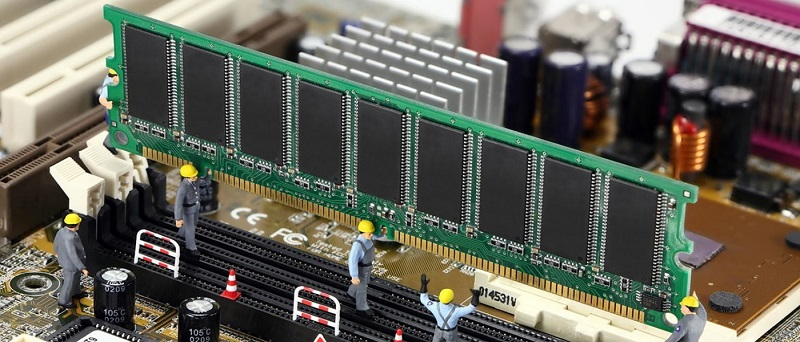
\includegraphics[width=6cm]{Memoria.jpg}
\centering
\caption{Memoria RAM}
\end{figure}

-Memoria ROM: Es la que se encarga de almacenar los datos de todas las aplicaciones y del sistema operativo.\newline

\begin{figure}[h]
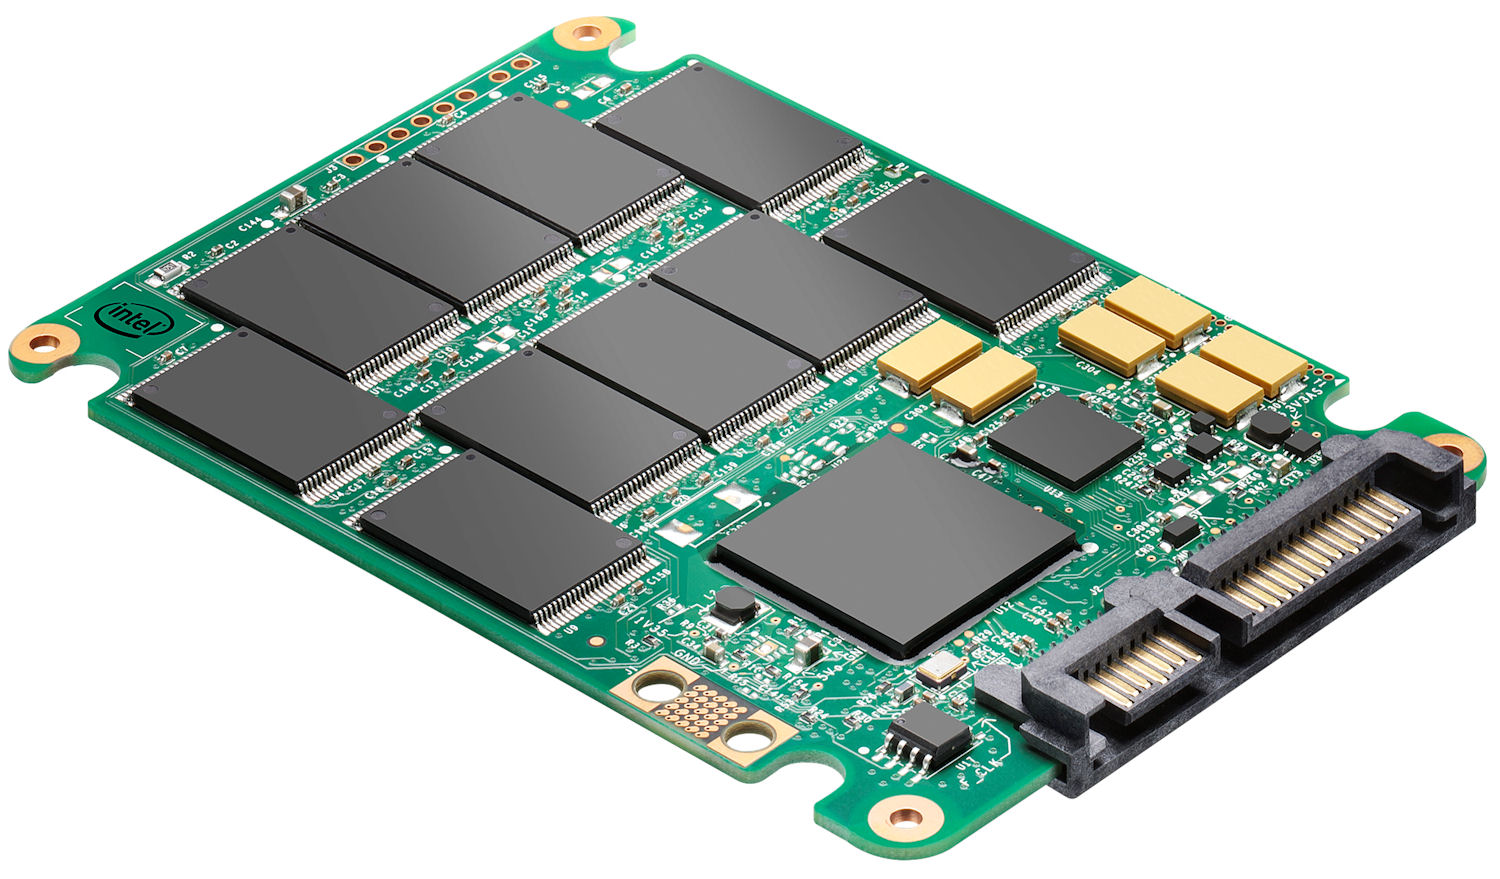
\includegraphics[width=6cm]{ssd.jpg}
\centering
\caption{Memoria ROM}
\end{figure}

-Memoria cache: Área de almacenamiento dedicada a los datos usados o solicitados con más frecuencia para su recuperación a gran velocidad, normalmente se ejecuta en el procesador \newline

\begin{figure}[h]
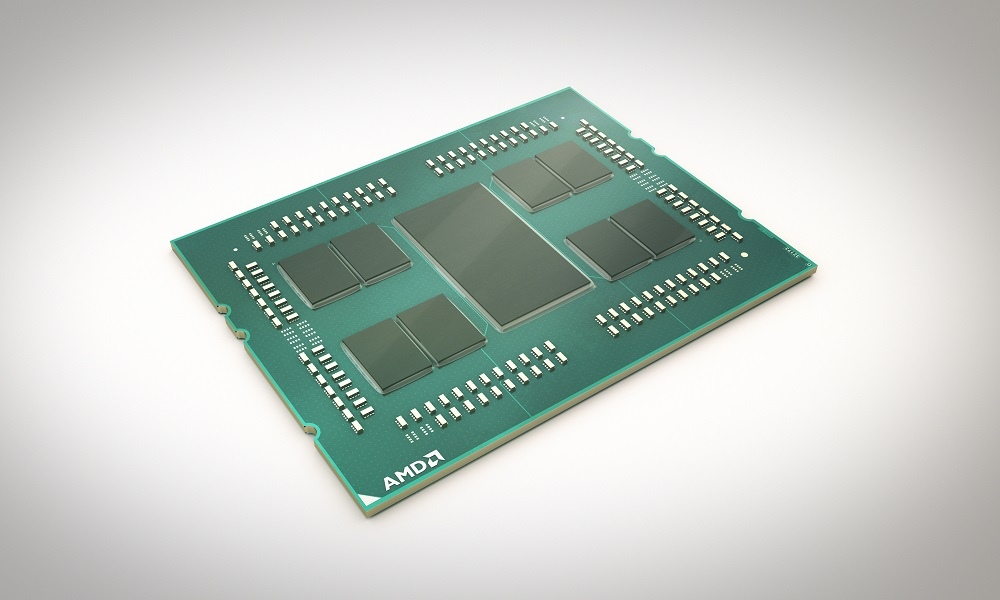
\includegraphics[width=6cm]{Cache.jpg}
\centering
\caption{Memoria cache}
\end{figure}

-Memoria DRAM: La memoria dinámica pierde su carga progresivamente, necesitando de un circuito dinámico de refresco que, cada cierto período, revisa dicha carga y la repone en un ciclo de refresco. \newline
\begin{figure}[h]
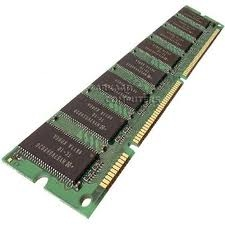
\includegraphics[width=4cm]{Dinamica.jpeg}
\centering
\caption{memoria DRAM}
\end{figure}

-Memoria SRAM: Basada en semiconductores, capaz de mantener los datos, mientras siga alimentada, sin necesidad de circuito de refresco. \newline
\begin{figure}[h]
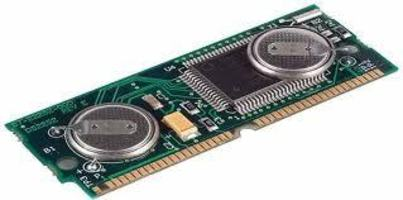
\includegraphics[width=6cm]{Estatica.jpg}
\centering
\caption{memoria SRAM}
\end{figure}

-Memoria Flash: Permite la lectura y escritura de datos, normalmente son portatiles debido a que son muy pequeñas. \newline
\begin{figure}[h]
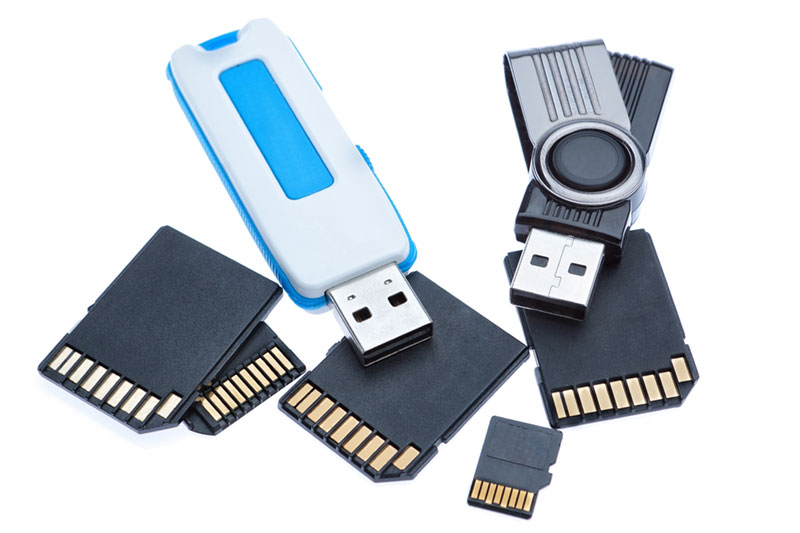
\includegraphics[width=6cm]{Flash.jpg}
\centering
\caption{memoria Flash}
\end{figure}

-Memoria Virtual: Es la memoria que se encarga de brindar tanto memoria para el usuario como para si misma, normalmente desde la unidad ROM \newline
\begin{figure}[h]
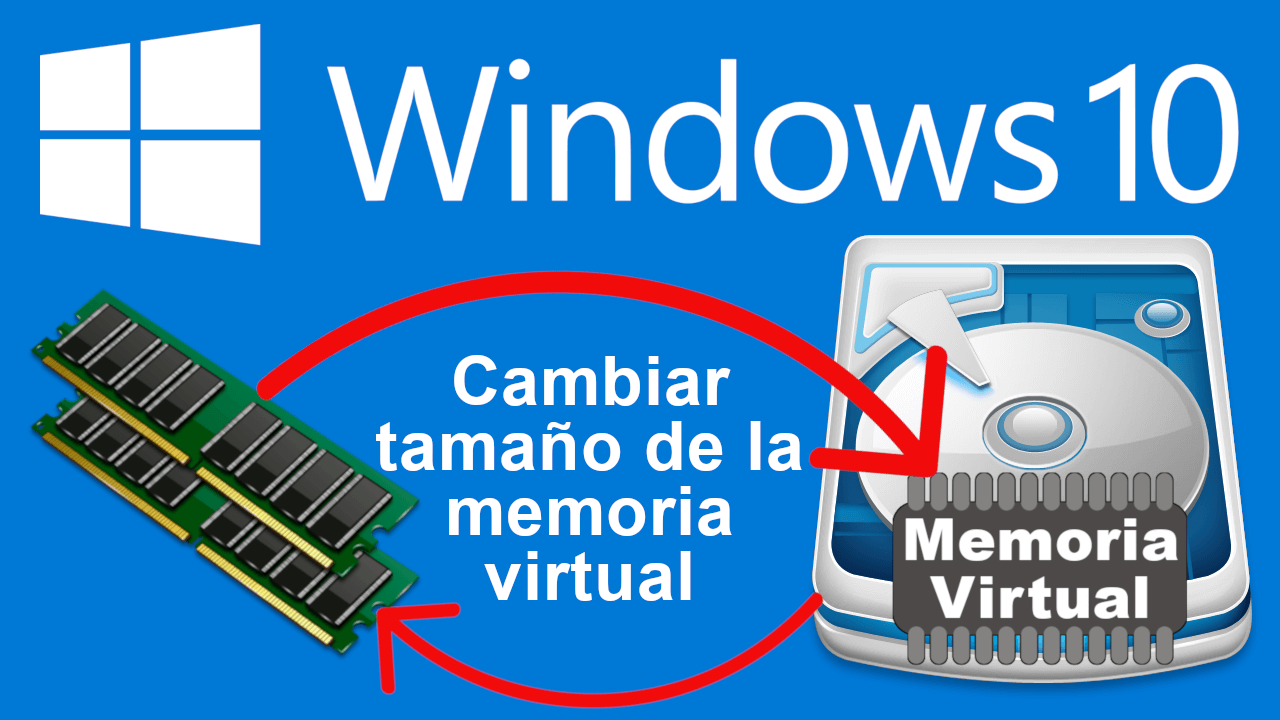
\includegraphics[width=6cm]{Virtual.png}
\centering
\caption{memoria Virtual}
\end{figure}

-Memoria VRAM: Es la memoria de video la cual permite ejecutar juegos, programas de alto nivel que requieran de muchos requisitos, en si es una memoria fundamental para un computador ya que es la que permite la alta calidad de imagen. \newline
\begin{figure}[h]
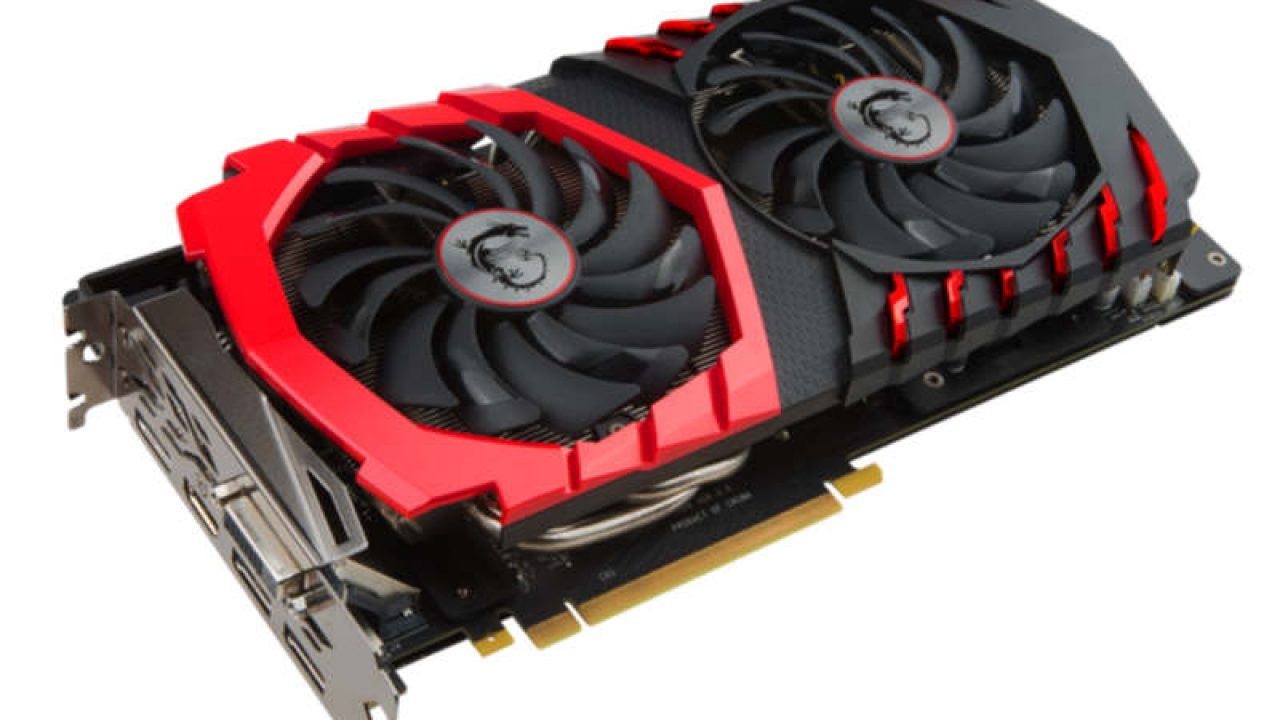
\includegraphics[width=4cm]{Vram.jpg}
\centering
\caption{memoria VRAM}
\end{figure}

\subsection{Describa la manera como se gestiona la memoria en un computador.}
1-Al iniciar el sistema operativo, los procesos de ejecucion del sistema se almacenan en el sistema \newline
2-Todos los programas se van a la memoria \newline
3-Se comienza un ciclo de abrir un programa y esté almacena sus datos en la memoria\newline
4-Cuando la memoria llena su capacidad de frecuencia, empieza a liberar datos o aplicaciones para disminuir espacio\newline
5-Vuelve a iniciar el ciclo de almacenamiento y liberar las secciones de memoria que ya no se utilizan para que estén disponibles para otros programas. \newline
6-Cuando se apaga el equipo, se borra toda la informacion de la memoria.\newline


\subsection{¿Qué hace que una memoria sea más rápida que otra? ¿Por qué esto es importante?}

Esto depende de muchos factores. \newline

Lo que hace rápido una memoria de otra es la frecuencia de lectura de datos, la velocidad determina la rapidez a la que es capaz de trabajar la memoria RAM y afecta, junto con el bus de datos, a su ancho de banda. Una mayor velocidad permite realizar transferencias en menos tiempo. Las operaciones de almacenar, borrar y Re almacenar nueva información y datos se completarán más rápidamente, lo que en algunos casos puede marcar una diferencia importante de rendimiento. También es muy importante la capacidad de la memoria debido a que, si una aplicación pide una alta capacidad de almacenamiento para sus datos y tenemos una memoria con poca capacidad, esté programa se ejecutara de manera incorrecta, pero si tenemos una memoria de alta capacidad no tendremos problemas para ejecutar ese mismo programa.


\section{Conclusión} \label{conclulsion}

Así mismo, sabiendo que tipo memorias existen y para que se utilizan, podemos decir que la memoria es el núcleo central de un computador, cabe decir que sin una memoria ningún equipo electrónico encendería ya que la memoria se encarga de distribuir información de un lugar a otro y también se encarga de almacenarla, por decirlo de una manera abstracta, la memoria es el cerebro del computador, eso quiere decir que es la que facilita que un computador realice diferentes operaciones simultáneamente. \newline


\bibliographystyle{IEEEtran}
\bibliography{references}
{
Tutorialspoint,
    author = "N.A",
    title = "ordenador - memoria",
    url  = "https://www.tutorialspoint.com/",
    addendum = "(N.N)",
    keywords = "Memoria" \newline
}
{
\newline muycomputer,
    author = "Isidro Ros",
    title = "Memoria RAM: qué es, por qué es importante y recomendaciones",
    url  = "https://www.muycomputer.com/2018/11/04/memoria-ram-que-es-recomendaciones/#:~:text=Una%20mayor%20velocidad%20permite%20realizar,una%20diferencia%20importante%20de%20rendimiento",
    addendum = "(4 noviembre, 2018)",
    keywords = "Memoria"
}


\end{document}
